 \section{Behavior}
In this section of the report, we will describe the behavior of the five classes from our class diagram. The sequence of events is not determined. On the sequence diagram of a problem figure \ref{fig:Klasse_diagram_problem}, the events "`detach problem"' can only happen after the event "`attach problem"' but it dose not show on the sequence diagram.      


\subsection{Problem}
\label{sub:problem}
Figure \ref{fig:Klasse_diagram_problem} shows the behavior of a problem. Note that you can solve the problem by attaching one or solutions. A problem can have an unlimited number of solutions. You can at all times delete the problem, thus the arrow points from the edge of the box.
\begin{figure}[H]
\begin{center}
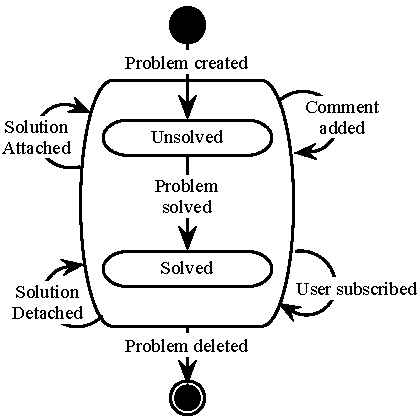
\includegraphics[scale=1]{input/problem_domain_analysis/Klassediagram_problem.pdf}
\caption{Statechart of a problem}
\label{fig:Klasse_diagram_problem}
\end{center}
\end{figure}

\subsection{Person}
As shown in figure \ref{fig:Klasse_diagram_person} a person is assigned a role in the system as soon as he is created. Thereafter multiple roles can be assigned to him.
\begin{figure}[H]
\begin{center}
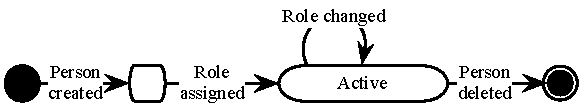
\includegraphics[scale=1]{input/problem_domain_analysis/Klassediagram_person.pdf}
\caption{Statechart of a problem}
\label{fig:Klasse_diagram_person}
\end{center}
\end{figure}
\begin{comment}
\subsection{List}
Figure \ref{fig:Klasse_diagram_list} shows the statechart of the list class. The list is a container of problems, and it can only exist within a department. We chose not to include the list as a class, as it was nothing but a container.
\begin{figure}[H]
\begin{center}
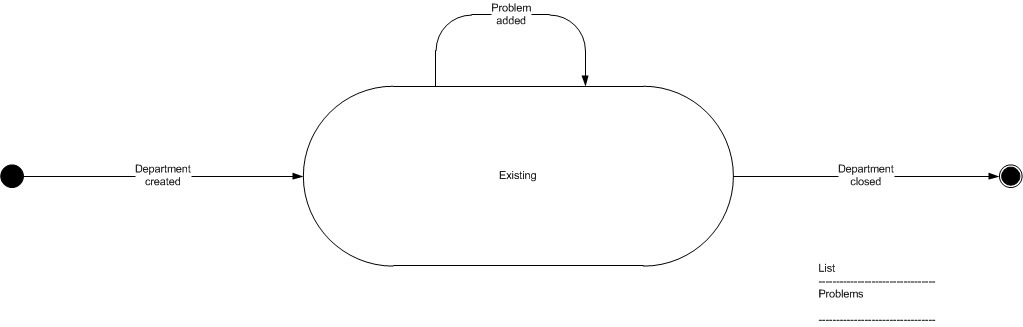
\includegraphics[width=1\textwidth]{input/problem_domain_analysis/Klassediagram_list.jpg}
\caption{Statechart of a list}
\label{fig:Klasse_diagram_list}
\end{center}
\end{figure}
\end{comment}

\subsection{Staff}
Figure \ref{fig:Klasse_diagram_staff} shows the statechart of the staff class. As shown on the Staff is a role to be assigned to persons. After a person receives that role, he or she can start receiving problem assignments. When all problems are either unassigned or solved, the person will be idle, meaning that the person is not doing anything useful with it's time. The role Staff can be unassigned only when there are no more problems assigned to that person.
\begin{figure}[H]
\begin{center}
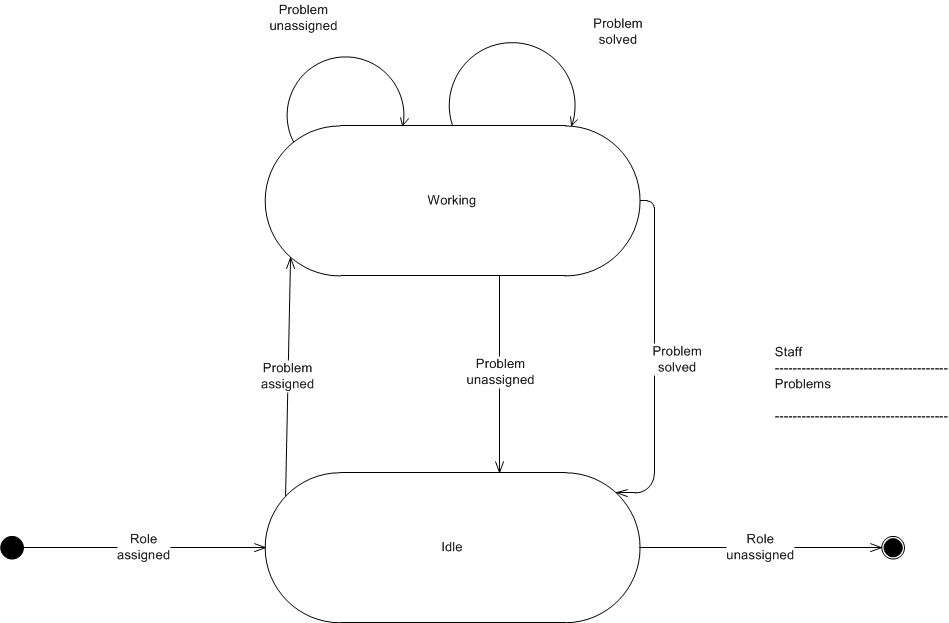
\includegraphics[width=1\textwidth]{input/problem_domain_analysis/Klassediagram_staff.jpg}
\caption{Statechart of a problem}
\label{fig:Klasse_diagram_staff}
\end{center}
\end{figure}

\subsection{User}
The statechart for a user consists of working state in which the user can create problems and comment on them. This is shown by figure \ref{fig:Klasse_diagram_user}.
\begin{figure}[H]
\begin{center}
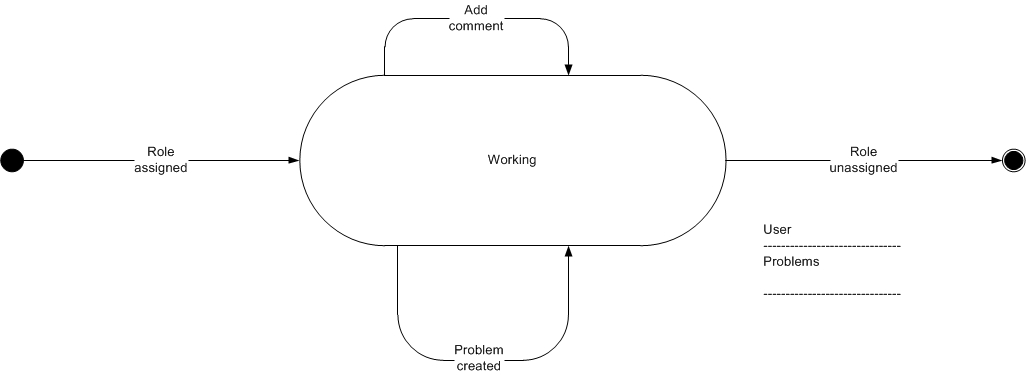
\includegraphics[width=1\textwidth]{input/problem_domain_analysis/Klassediagram_user.jpg}
\caption{Statechart of a problem}
\label{fig:Klasse_diagram_user}
\end{center}
\end{figure}

\subsection{Department}
As shown in figure \ref{fig:Klasse_diagram_department} can be open, after which staff can be both hired and fired. A department exists untill it is closed.
\begin{figure}[H]
\begin{center}
\includegraphics[scale=1]{input/problem_domain_analysis/klassediagram_department.pdf}
\caption{Statechart of a problem}
\label{fig:Klasse_diagram_department}
\end{center}
\end{figure}